\documentclass[11pt]{article}
\usepackage{fancyhdr,url,graphicx,courier,xcolor,multicol,shadethm}
\usepackage[top=1in,bottom=1in,left=0.75in,right=0.75in,headheight=.75in]{geometry}
\usepackage[small,bf]{caption}
\definecolor{shadethmcolor}{rgb}{0.96,0.96,0.96}
\pagestyle{fancy}
\lhead{T.~Keller, Y.~Tan, K.~Huang, and C.~Li}
\rhead{CSCI 6360 Group Project}
\cfoot{\thepage/\pageref{LastPage}}
\frenchspacing
%%%%%%%%%%%%%%%%%%%%%%%%%%%%%%%%%%%%%%%%%%%%%%%%%%%%%%%%%%%%%%%%%%%%%%%%%%%%%%%%%%%%%%%%%%%%%%%%%%%%
\definecolor{codebg}{gray}{0.8}
\renewcommand{\headrulewidth}{0.01in} \renewcommand{\footrulewidth}{0.01in}
\newcommand{\code}[1]{\colorbox{codebg}{\texttt{\footnotesize{#1}}}}
%%%%%%%%%%%%%%%%%%%%%%%%%%%%%%%%%%%%%%%%%%%%%%%%%%%%%%%%%%%%%%%%%%%%%%%%%%%%%%%%%%%%%%%%%%%%%%%%%%%%
\begin{document}
\centerline{\large{\bfseries MMSP Compute and I/O Performance on AMOS}}
\begin{multicols}{4}\centering
 \textbf{Trevor Keller}\\
 \emph{Materials Science}
 
 \textbf{Yixuan Tan}\\
 \emph{Mechanical Engineering}

 \textbf{Kun Huang}\\
 \emph{Physics}
 
 \textbf{Congrui Li}\\
 \emph{Computer Science}

\end{multicols}

\begin{center}
\texttt{\{kellet,tany3,huangk4,lic10\}@rpi.edu}

\vskip\baselineskip
Rensselaer Polytechnic Institute\\110 Eighth Street\\Troy, NY 12180

\vskip\baselineskip
May 8, 2014
\end{center}


\begin{abstract}
The Mesoscale Microstructure Simulation Project (MMSP) is a C++ code for parallel simulation of systems of interest in materials science using kinetic Monte Carlo, phase-field, and similar methods.\footnote{\url{http://matforge.org/mmsp} and \url{http://github.com/mesoscale/mmsp}}
To date, MMSP has been tested and used extensively on workstation-class machines, occasionally on clusters (such as the CCI Opteron cluster), and almost never on supercomputers.
The primary obstacle to using MMSP on AMOS, CCI's Blue Gene/Q, is its parallel I/O performance:
while the calculations finish, either the program locks up when writing to disk, or large chunks of the data are never written.
\end{abstract}

\begin{multicols}{2}
\section{Introduction}
The Mesoscale Microstructure Simulation Project (MMSP, \url{http://matforge.org/mmsp} and \url{http://github.com/mesoscale/mmsp}) is a C++ code for parallel simulation of systems of interest in materials science using kinetic Monte Carlo, phase-field, and similar methods.
MMSP implements a 3-dimensional grid class, with back-end support for parallel synchronization and file I/O using MPI.
This grid facilitates computation of spatial derivatives by exchanging ``ghost'' cells between spatially adjacent ranks:
essentially, each face of the local 3-D grid needs to be sent to the MPI rank sharing that face.
This is a common feature of codes for numerical integration of partial differential equations;
indeed, while designed for materials science, MMSP could be applicable to a large number of numerical computing tasks.
Like the matrix multiplication program beaten to death in class, MMSP presents a strong-scaling problem:
the grid size (like a 3-D matrix) is fixed; adding more processors does not change the global problem, only the amount of work each rank must complete.

To date, MMSP has been tested and used extensively on workstation-class machines, occasionally on clusters (such as the CCI Opteron cluster), and almost never on supercomputers.
The primary obstacle to using MMSP on the AMOS, CCI's Blue Gene/Q, is its parallel I/O performance:
while the calculations finish, either the program locks up when writing to disk, or large chunks of the data are never written.

Past efforts at MPI-IO have used \texttt{MPI::File::Iwrite\_shared}, \texttt{MPI::File::Iwrite\_at}, and \texttt{MPI::File::Write\_at\_all}.
However, the code has never taken the underlying filesystem into consideration.
On AMOS, the GPFS has a blocksize of 8MB, while the MPI ranks may only write a few KB each.
This produces contention for a common GPFS block between thousands of processors!
Efforts are underway to implement a two-stage accumulate-and-write output strategy, wherein a few MPI ranks gather data from the upstream ranks that would contend for the same block;
only the accumulator ranks write to disk, once their output buffers are full.

In addition to the grid class, MMSP provides a number of example cases for scientifically interesting problems.
These are typically computationally demanding, with many floating-point operations to perform for each voxel in the grid.
The second goal of this group project is to use POSIX threads in MMSP to improve numerical performance (FLOPS).

Two examples of simulated grain growth -- one using kinetic Monte Carlo, the other phase-field -- will be chosen for comparison.
The explicit solver will be upgraded to spawn up to 4 \texttt{pthreads} per MPI rank.
Each code will write the data to disk after a set number of Monte Carlo Steps or Phase-Field Iterations.
The execution time, compute time, and IO time will be recorded, and performance will be computed in terms of FLOPS, memory bandwidth, and disk bandwidth.
These measurements will form the basis for a write-up benchmarking the performance of the AMOS Blue Gene/Q and its GPFS filesystem.
We intend to repeat these tests using up to 512 nodes on AMOS, and to produce a publication-quality report from this work.

\section{Algorithms}

\subsection*{Potts Monte Carlo}
The overall grid is portioned in to different local grids so that each processor is assigned a contiguous subgrid.
In two dimensions this is a small rectangular section, and in three dimensions it is a rectangular box.
Each processor also stores a copy of the narrow strips (or planes in three dimensions) of lattice sites that immediately adjoin its sub-domain and which are actually owned by neighboring processors.
This allows a processor to check neighboring spin values of sites on the edge of its sub-domain.
With these data structures, every processor can now simultaneously flip spins in its sub-domain without violating the rule of detailed balance, 
so long as one processor does not choose a lattice site on an edge of its sub-domain at the same time the processor adjoining that edge does likewise.
We enforce this restriction in our parallel Potts algorithm by ``slicing'' the subgrid as shown in Figure 1. 
lattice site is represented by a square (not the corners of the square) and assigned a ``sublattice'' number, 0 or 1.

\begin{minipage}{0.45\textwidth}\centering
  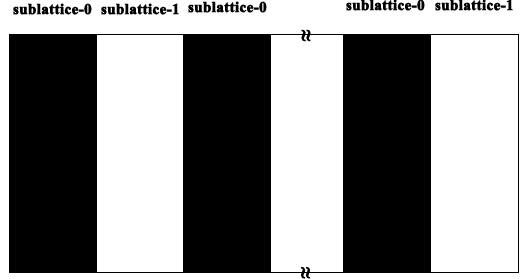
\includegraphics[height=1.5in]{mc-fig-01}
  \captionof{figure}{Slicing subgrid into sublattice used for parallel Potts grain growth algorithm.\label{fig:mc1}}
\end{minipage}



A subgrid is divided into sublattices as in Figure l, where only the lattice sites assigned to sublattice-0 are now shown as shaded.
The key point is that the 2 neighbors of a sublattice-0 lattice site do not include any other sublattice-0 lattice sites.
The parallel Monte Carlo Potts grain growth algorithm for one sweep can now be written as follows:
\begin{minipage}{0.45\textwidth}\centering
\begin{shadebox}
\begin{itemize}
  \item Loop over sublattice (i)
  \begin{itemize}
    \item Loop over all lattice sites of sublattice $i$\\ within my subgrid
    \begin{itemize}
      \item Pick a new spin value randomly.
      \item Compute the energy change for the site\\ to change to the new spin.
      \item Accept or reject the change based on\\ the Boltzmann criterion.
    \end{itemize}
    \item[*] End lattice site loop
    \item Exchange sites along edge of my subgrid with\\ neighboring processors to acquire current\\ neighbor spin values.
    \end{itemize}
    \item[*] End color loop
\end{itemize}
\end{shadebox}
\end{minipage}

This algorithm works for both 2-D and 3-D lattices. Also, the communication of subgrid ``edges'' becomes ``planes'' in 3-D. 

\begin{minipage}{0.45\textwidth}\centering
  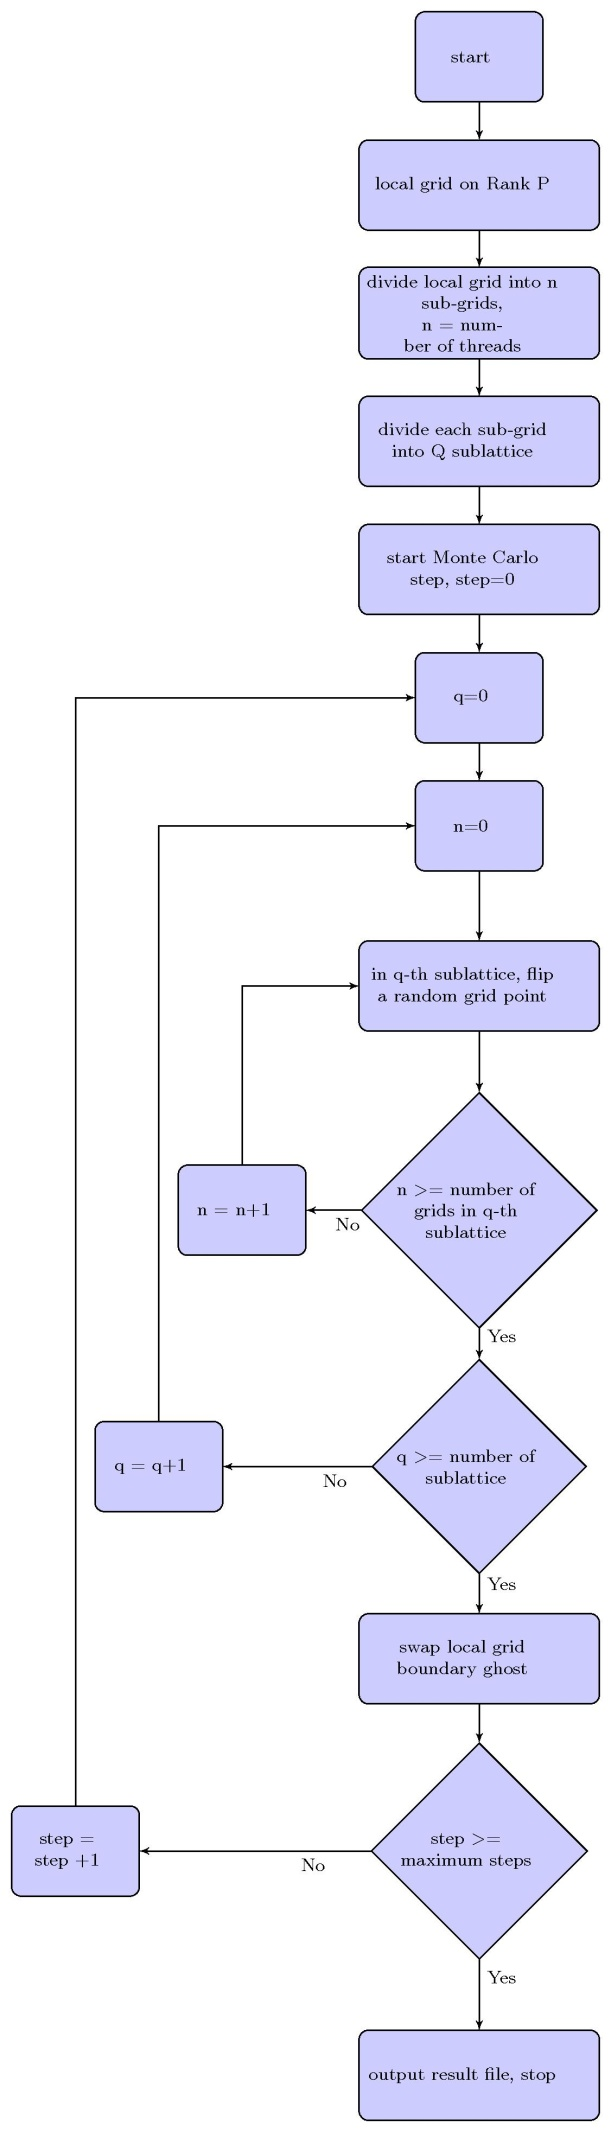
\includegraphics[height=0.95\textheight]{mc-fig-02}
  \captionof{figure}{\emph{No caption provided.}\label{fig:mc2}}
\end{minipage}

\subsection*{Phase-Field}

\label{LastPage}
\end{multicols}
\end{document}
